\chapter{Computing with particles}
\label{app:computing-with-particles}

\phantom{\gps{}\gps{}\gps{}}

The particle filter allows us to approximate any distribution by using a sample of \emph{particles}, $x\vi$, with weights $w\vi$. There are many advantages of the particle filter, but one is that producing summary statistics is very simple. The only real disadvantage is that it is a computationally demanding process. In this appendix, I briefly describe the theory behind using the particle filter to estimate a distribution, as well as give details on its computational demands.


\section{The Dirac measure}
\label{app:dirac-delta-measure}

In \cref{sec:recursive-bayes,cha:vehicle_model} I described the particle filter implementation, and noted that we can use the Dirac measure, $\dirac$, to approximate the distribution \citep{Benedetto_1996}. We will not get into the theoretical aspects of the function, except to state the following property:
\begin{equation}
\label{eq:dirac_property}
\int_X f(x) \dirac_y(x)\dx = f(y).
\end{equation}

Let $x$ be an unknown quantity for which we have a sample of $N$ particles $\{x\vi\}_{i=1}^N$ with associated weights $\{w\vi\}_{i=1}^N$. The Dirac delta measure allows the approximation of the distribution of $x$ as
\begin{equation}
\label{eq:dirac_dist}
p(x) \approx \sum_{i=1}^N w\vi \dirac_{x\vi}(x).
\end{equation}


Using \cref{eq:dirac_property,eq:dirac_dist} we can now compute, for example, the mean, using $f(x) = x$,
\begin{equation}
\label{eq:dirac_mean}
\begin{split}
\bar x &= \int_X x p(x) \dx \\
&= \int_X x \sum_{i=1}^N w\vi \dirac_{x\vi}(x) \dx \\
&= \sum_{i=1}^N w\vi \int_X x \dirac_{x\vi}(x) \dx \\
&= \sum_{i=1}^N w\vi x\vi.
\end{split}
\end{equation}



\section{Calculating particle coordinates}
\label{app:pf_measurement_fun}

An important aspect of the model used in \cref{cha:vehicle_model} is the \emph{measurement function}. I mentioned that we are able to obtain \gls{gps} coordinates for individual particles, allowing us to compare them directly to the observation. Doing so requires first that we have a \emph{shape path} consisting of a sequence of coordinates (as shown in \cref{fig:app:route_shape}), for which we can compute the distance between each. This, in turn, allows us to compute the \emph{cumulative distance} of each point within the shape, referred to as \emph{shape distance travelled} (in meters).

\begin{knitrout}\small
\definecolor{shadecolor}{rgb}{0.969, 0.969, 0.969}\color{fgcolor}\begin{figure}[h]

{\centering 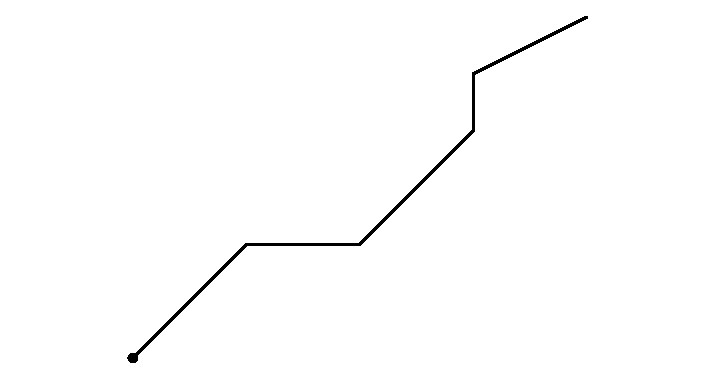
\includegraphics[width=.6\textwidth]{figure/app:route_shape-1} 

}

\caption[A shape path, starting at the point (lower left)]{A shape path, starting at the point (lower left).}\label{fig:app:route_shape}
\end{figure}


\end{knitrout}

To find the coordinates of a point 40~meters along this line, we find the maximum point along the route with \emph{shape distance travelled} less than 40, which is the point in red in \cref{fig:app:measure_step1}, which is 31~meters along the route. There remains $40-31=9$~meters to travel to get to 40~meters.

\begin{knitrout}\small
\definecolor{shadecolor}{rgb}{0.969, 0.969, 0.969}\color{fgcolor}\begin{figure}[ht]

{\centering 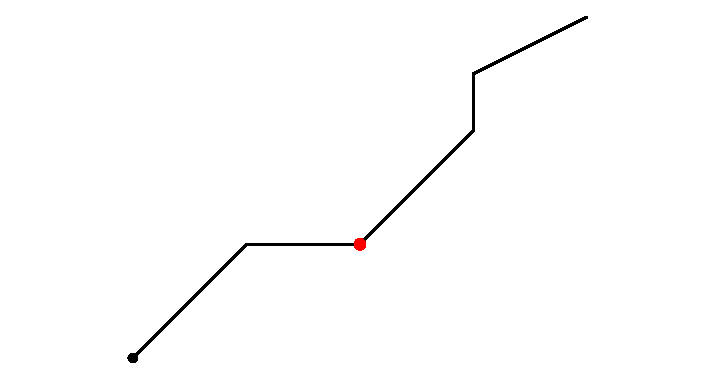
\includegraphics[width=.6\textwidth]{figure/app:measure_step1-1} 

}

\caption[The farthest point along the route less than 40~meters along the route (red)]{The farthest point along the route less than 40~meters along the route (red).}\label{fig:app:measure_step1}
\end{figure}


\end{knitrout}

To compute the desired coordinates, we use the \emph{destination point} formula, which takes a start point, bearing, and distance to travel and returns a final point. The function \verb+destPoint()+ is available in the \pkg{geosphere} package \citep{geosphere}. The \emph{bearing} required is shown in \cref{fig:app:measure_step2}:

\begin{knitrout}\small
\definecolor{shadecolor}{rgb}{0.969, 0.969, 0.969}\color{fgcolor}\begin{figure}[h]

{\centering 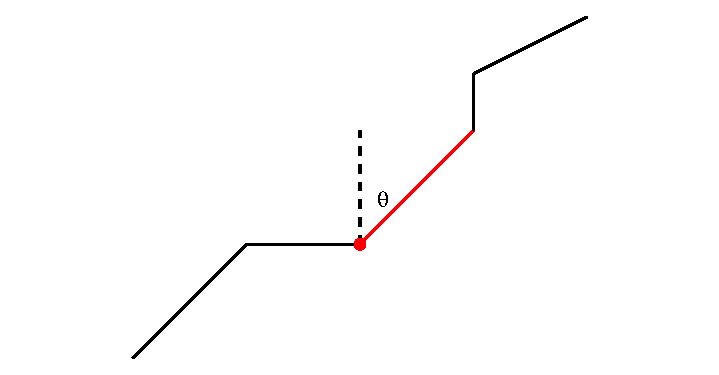
\includegraphics[width=.6\textwidth]{figure/app:measure_step2-1} 

}

\caption[The bearing, $\theta$, is the angle between the dashed line (North) and the red line]{The bearing, $\theta$, is the angle between the dashed line (North) and the red line.}\label{fig:app:measure_step2}
\end{figure}


\end{knitrout}

Travelling 9~meters from the red point at a bearing of $\theta^\circ$ (degrees) yields the \gls{gps} coordinates of the particle $x=40$~meters along the route, indicated by the point in \cref{fig:app:measure_step3} below, and is calculated using the \pkg{geosphere} package:
\begin{knitrout}\small
\definecolor{shadecolor}{rgb}{0.969, 0.969, 0.969}\color{fgcolor}\begin{kframe}
\begin{alltt}
\hlstd{particle_coord} \hlkwb{<-} \hlstd{geosphere}\hlopt{::}\hlkwd{distGeo}\hlstd{(start, bearing, dist)}
\end{alltt}
\end{kframe}
\end{knitrout}

\begin{knitrout}\small
\definecolor{shadecolor}{rgb}{0.969, 0.969, 0.969}\color{fgcolor}\begin{figure}[h]

{\centering 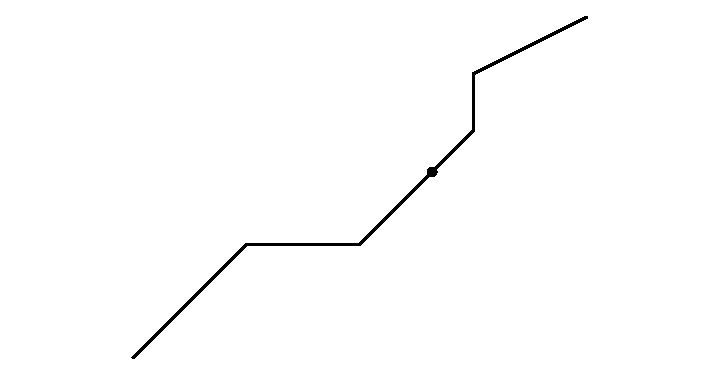
\includegraphics[width=.6\textwidth]{figure/app:measure_step3-1} 

}

\caption[The final position of the particle is obtained by travelling 19~meters along the red line]{The final position of the particle is obtained by travelling 19~meters along the red line.}\label{fig:app:measure_step3}
\end{figure}


\end{knitrout}

\section{Resampling}
\label{app:particle-resampling}

Part of the particle filter update step is to, when required, resample the particles according to their weights. This involves generating random numbers to determine which particles to include in the sample, replacing the vector of particle states with the new sample. The latter is straightforward: we simply copy the sampled particles into a new vector and, once finished, replace the original vector with the new one.


We will now describe unweighted resampling first before discussing weighted. Given a sample of size $N$, we use a \gls{rng} to obtain uniform numbers $u \in (0, 1)$. Since each particle has equal weight, we multiply $u$ by $N$ and round down (using the \emph{floor} function), to get
\begin{equation}
j = \lfloor uN \rfloor.
\end{equation}
Thus, we have sampled particle $j$.


When the particles are weighted, however, we cannot simply use $uN$. For example, here we have five particles, where each is represented by a rectangle whose width is equal to the particle's weight (the total weight is unity), as shown in \cref{fig:app_weighted_resampling}.
\begin{knitrout}\small
\definecolor{shadecolor}{rgb}{0.969, 0.969, 0.969}\color{fgcolor}\begin{figure}[h]

{\centering 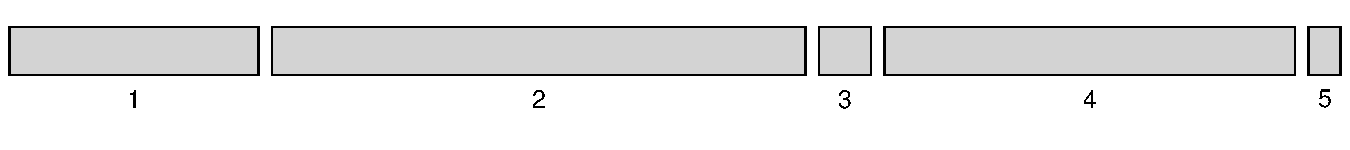
\includegraphics[width=0.8\textwidth]{figure/app_weighted_resampling-1} 

}

\caption[Visualisation of cumulative particle weights as used during resampling]{Visualisation of cumulative particle weights as used during resampling.}\label{fig:app_weighted_resampling}
\end{figure}


\end{knitrout}

As before, we use a \gls{rng} to obtain a uniform random number $u$; to map the number to a particle, we compute \emph{cumulative weights} and find the first particle with cumulative weight greater than $u$:
\begin{equation}
j = \min\left\{k = 1, \ldots, N : \sum_{i=1}^k w\vi[i] \geq u\right\}.
\end{equation}




\section{Summary statistics}
\label{app:particle-summaries}

Another core part of the program is computing of summary statistics, for example the mean and variance. However, these are easily computed using \verb+std::accumulate+, for example, a vehicle's mean speed is obtained by:
\begin{lstlisting}
double mean = std::accumulate (
    x.begin (), x.end (),
    // initial value
    0.,
    // lambda function, where 'a' is the current value
    [](double a, Particle& p) {
        return a + p.get_weight () * p.get_speed ();
    }
);
\end{lstlisting}
Similarly, the variance can be calculated by passing a reference to the value of {\tt mean} to the lambda function (within {\tt []}), which becomes
\begin{lstlisting}
[&mean](double a, Particle& p) {
    return a + p.get_weight () * pow (p.get_speed () - mean, 2.);
}
\end{lstlisting}

More complicated, however, is estimation of \emph{quantiles}, since this requires sorting the vector of particles in order of the desired value. In the above example, to get the median speed, we need to first sort the particles by speed (slowest to fastest) and then sum their weights, in order, until the sum exceeds 0.5: the speed of the particle that does this provides the median speed.
\begin{lstlisting}
std::sort (x.begin (), x.end (),
    (Particle& p1, Particle& p2)
    {
        return p1.get_speed () < p2.get_speed ();
    }
);
double wt = 0.;
int i = 0;
while (wt < 0.5) wt += x.at (i++).get_weight ();
double median = x.at (i).get_speed ();
\end{lstlisting}

The issue here is the first step, sorting, which has computational complexity of $\mathcal{O}(N\log N)$.\footnote{Described on the documentation page for \texttt{std::sort}, \url{https://en.cppreference.com/w/cpp/algorithm/sort}.} If we wish to estimate the median distance and the median speed, we need to sort the particles \emph{twice}. In \cref{cha:etas}, we used multiple quantiles for each stop: this requires sorting each vehicle's particles once for each upcoming stop. However, since we use a subsample to compute \glspl{eta} ($N^\star$), the complexity is significantly less, $\mathcal{O}(N^\star\log N^\star)$; if we attempted to use all $N$ particles (in the simulation used in \cref{cha:prediction}, we used $N=10000$) the application would have taken far longer.



\section{Calculating ETA CDFs}
\label{app:particle-eta-cdf}

It is also possible to summarize the \gls{cdf} by using the definition in \cref{eq:particle_eta_modulus,eq:pf_pdf_arrivaltime,eq:pf_cdf_arrivaltime} (starting on \cpageref{eq:particle_eta_modulus}) and rounding estimates to minutes. This is the equivalent of computing the modules of an \gls{eta} in seconds with 60. Then we simply tally the number of particles with each \gls{eta}, which is straightforward in \Cpp{} by incrementing the \verb+eta+th index of the \gls{eta} vector.


\begin{lstlisting}
int Amax, eta;
std::vector<int> cdf;
Amax = std::max (state.begin (); state.end ();
    [](Particle& p) { return p.arrival_times.at (stop_index) % 60; });

// create vector as long as max ETA and set all values to 0:
cdf.resize (Amax, 0);

for (auto p : state)
{
    eta = p.arrival_times.at (stop_index) % 60;
    cdf[eta]++;
}
\end{lstlisting}
